\begin{quote}
This is part 29 of Categories for Programmers. Previously: {Enriched
Categories}. See the
\href{https://bartoszmilewski.com/2014/10/28/category-theory-for-programmers-the-preface/}{Table
of Contents}.
\end{quote}

I realize that we might be getting away from programming and diving into
hard-core math. But you never know what the next big revolution in
programming might bring and what kind of math might be necessary to
understand it. There are some very interesting ideas going around, like
functional reactive programming with its continuous time, the extention
of Haskell's type system with dependent types, or the exploration on
homotopy type theory in programming.

So far I've been casually identifying types with \emph{sets} of values.
This is not strictly correct, because such approach doesn't take into
account the fact that, in programming, we \emph{compute} values, and the
computation is a process that takes time and, in extreme cases, might
not terminate. Divergent computations are part of every Turing-complete
language.

There are also foundational reasons why set theory might not be the best
fit as the basis for computer science or even math itself. A good
analogy is that of set theory being the assembly language that is tied
to a particular architecture. If you want to run your math on different
architectures, you have to use more general tools.

One possibility is to use spaces in place of sets. Spaces come with more
structure, and may be defined without recourse to sets. One thing
usually associated with spaces is topology, which is necessary to define
things like continuity. And the conventional approach to topology is,
you guessed it, through set theory. In particular, the notion of a
subset is central to topology. Not surprisingly, category theorists
generalized this idea to categories other than \textbf{Set}. The type of
category that has just the right properties to serve as a replacement
for set theory is called a \emph{topos} (plural: topoi), and it
provides, among other things, a generalized notion of a subset.

\subsection{Subobject Classifier}\label{subobject-classifier}

Let's start by trying to express the idea of a subset using functions
rather than elements. Any function \texttt{f} from some set \texttt{a}
to \texttt{b} defines a subset of \texttt{b}--that of the image of
\texttt{a} under \texttt{f}. But there are many functions that define
the same subset. We need to be more specific. To begin with, we might
focus on functions that are injective --- ones that don't smush multiple
elements into one. Injective functions ``inject'' one set into another.
For finite sets, you may visualize injective functions as parallel
arrows connecting elements of one set to elements of another. Of course,
the first set cannot be larger than the second set, or the arrows would
necessarily converge. There is still some ambiguity left: there may be
another set \texttt{a\&apos;} and another injective function
\texttt{f\&apos;} from that set to \texttt{b} that picks the same
subset. But you can easily convince yourself that such a set would have
to be isomorphic to \texttt{a}. We can use this fact to define a subset
as a family of injective functions that are related by isomorphisms of
their domains. More precisely, we say that two injective functions:

\begin{verbatim}
f :: a -> b f&apos;:: a&apos;-> b
\end{verbatim}

are equivalent if there is an isomorphism:

\begin{verbatim}
h :: a -> a&apos;
\end{verbatim}

such that:

\begin{verbatim}
f = f&apos; . h
\end{verbatim}

Such a family of equivalent injections defines a subset of \texttt{b}.

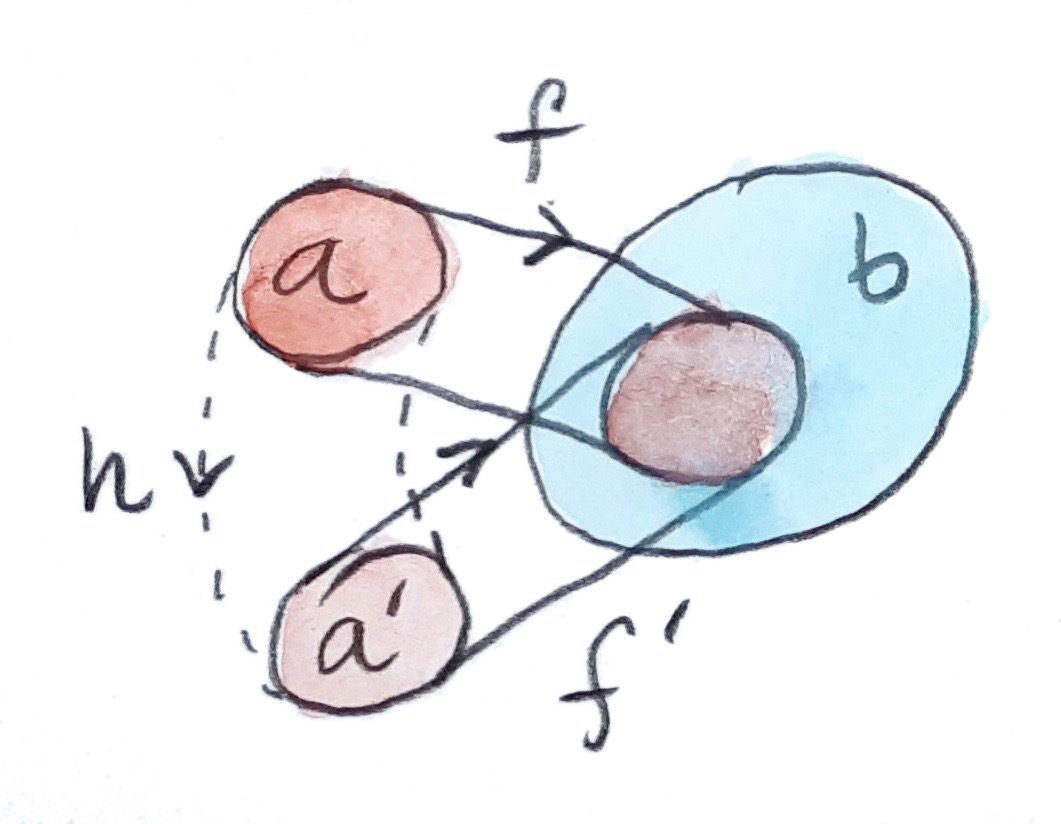
\includegraphics[width=2.29167in]{images/subsetinjection.jpg}

This definition can be lifted to an arbitrary category if we replace
injective functions with monomorphism. Just to remind you, a
monomorphism \texttt{m} from \texttt{a} to \texttt{b} is defined by its
universal property. For any object \texttt{c} and any pair of morphisms:

\begin{verbatim}
g :: c -> a g&apos;:: c -> a
\end{verbatim}

such that:

\begin{verbatim}
m . g = m . g&apos;
\end{verbatim}

it must be that \texttt{g\ =\ g\&apos;}.

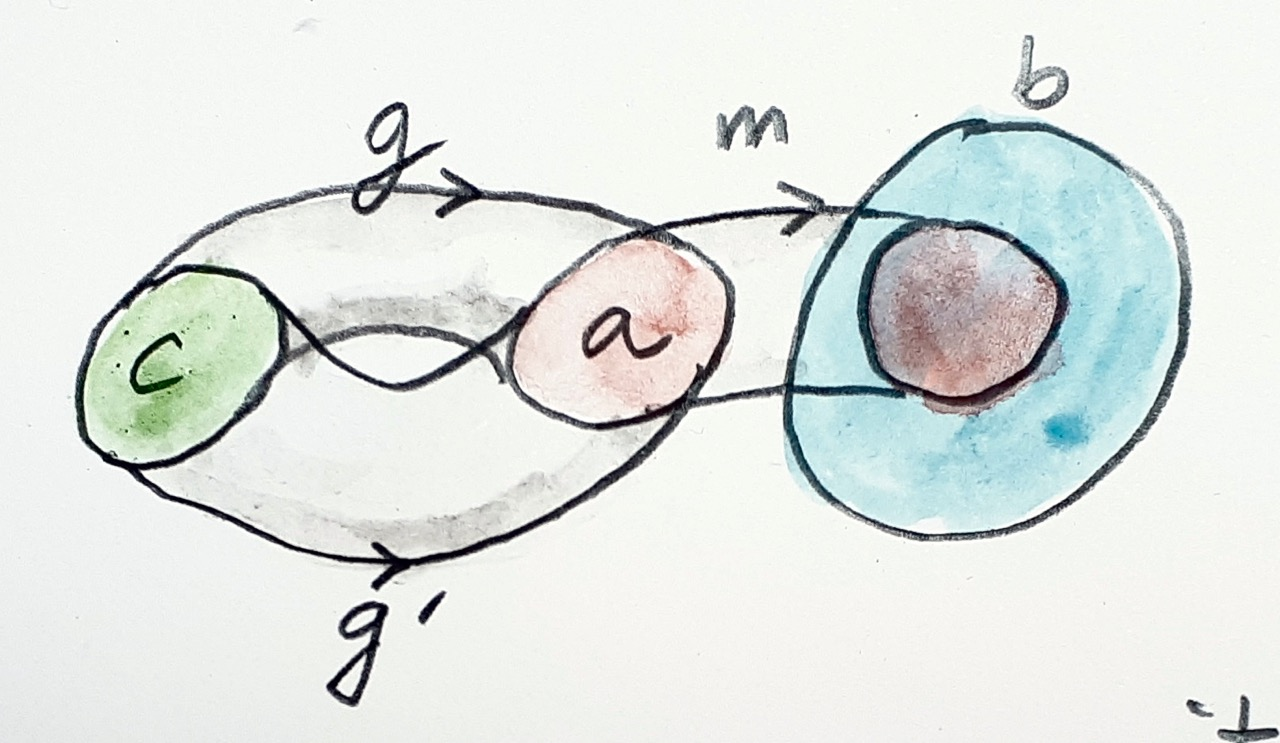
\includegraphics[width=3.12500in]{images/monomorphism.jpg}

On sets, this definition is easier to understand if we consider what it
would mean for a function \texttt{m} \emph{not} to be a monomorphism. It
would map two different elements of \texttt{a} to a single element of
\texttt{b}. We could then find two functions \texttt{g} and
\texttt{g\&apos;} that differ only at those two elements. The
postcomposition with \texttt{m} would then mask this difference.

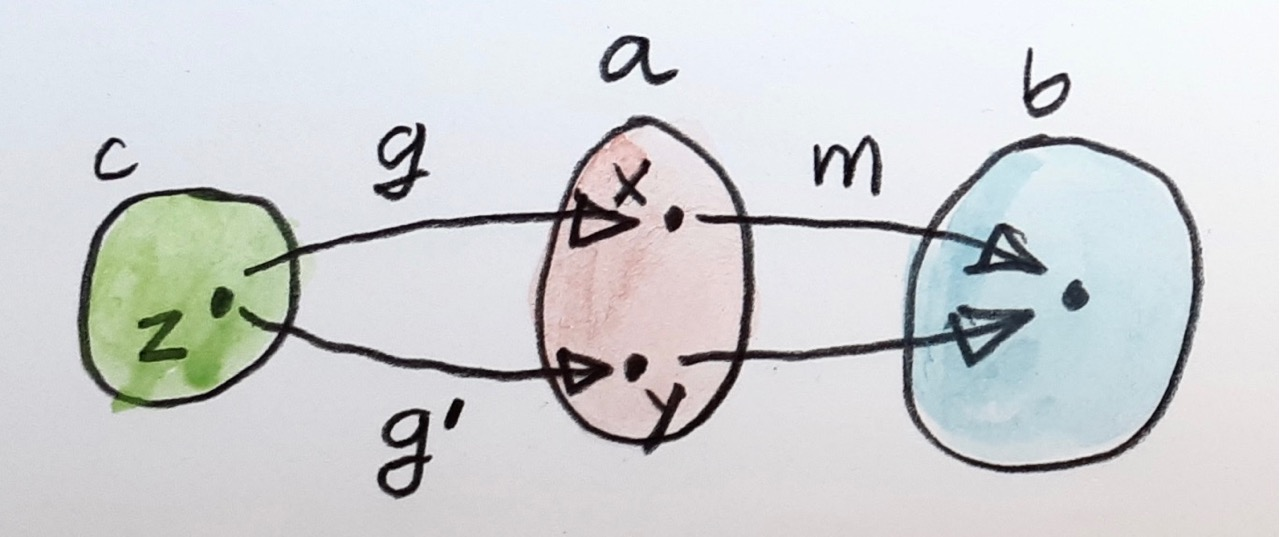
\includegraphics[width=3.12500in]{images/notmono.jpg}

There is another way of defining a subset: using a single function
called the characteristic function. It's a function \texttt{χ} from the
set \texttt{b} to a two-element set \texttt{Ω}. One element of this set
is designated as ``true'' and the other as ``false.'' This function
assigns ``true'' to those elements of \texttt{b} that are members of the
subset, and ``false'' to those that aren't.

It remains to specify what it means to designate an element of
\texttt{Ω} as ``true.'' We can use the standard trick: use a function
from a singleton set to \texttt{Ω}. We'll call this function
\texttt{true}:

\begin{verbatim}
true :: 1 -> Ω
\end{verbatim}

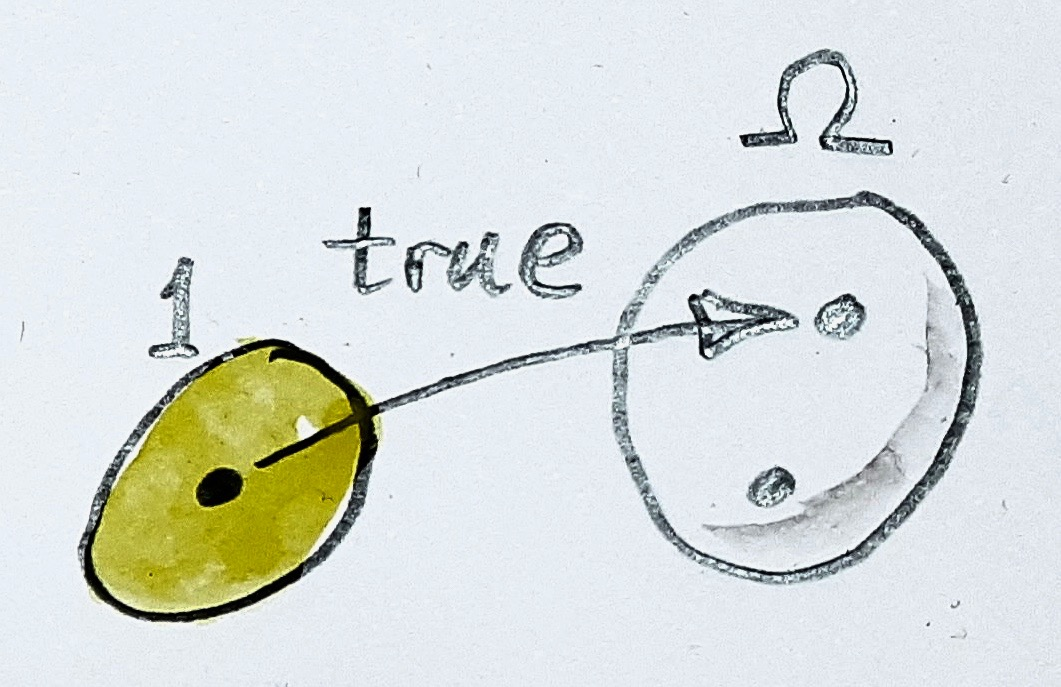
\includegraphics[width=1.97917in]{images/true.jpg}

These definitions can be combined in such a way that they not only
define what a subobject is, but also define the special object
\texttt{Ω} without talking about elements. The idea is that we want the
morphism \texttt{true} to represent a ``generic'' subobject. In
\textbf{Set}, it picks a single-element subset from a two-element set
\texttt{Ω}. This is as generic as it gets. It's clearly a proper subset,
because \texttt{Ω} has one more element that's \emph{not} in that
subset.

In a more general setting, we define \texttt{true} to be a monomorphism
from the terminal object to the \emph{classifying object} \texttt{Ω}.
But we have to define the classifying object. We need a universal
property that links this object to the characteristic function. It turns
out that, in \textbf{Set}, the pullback of \texttt{true} along the
characteristic function \texttt{χ} defines both the subset \texttt{a}
and the injective function that embeds it in \texttt{b}. Here's the
pullback diagram:

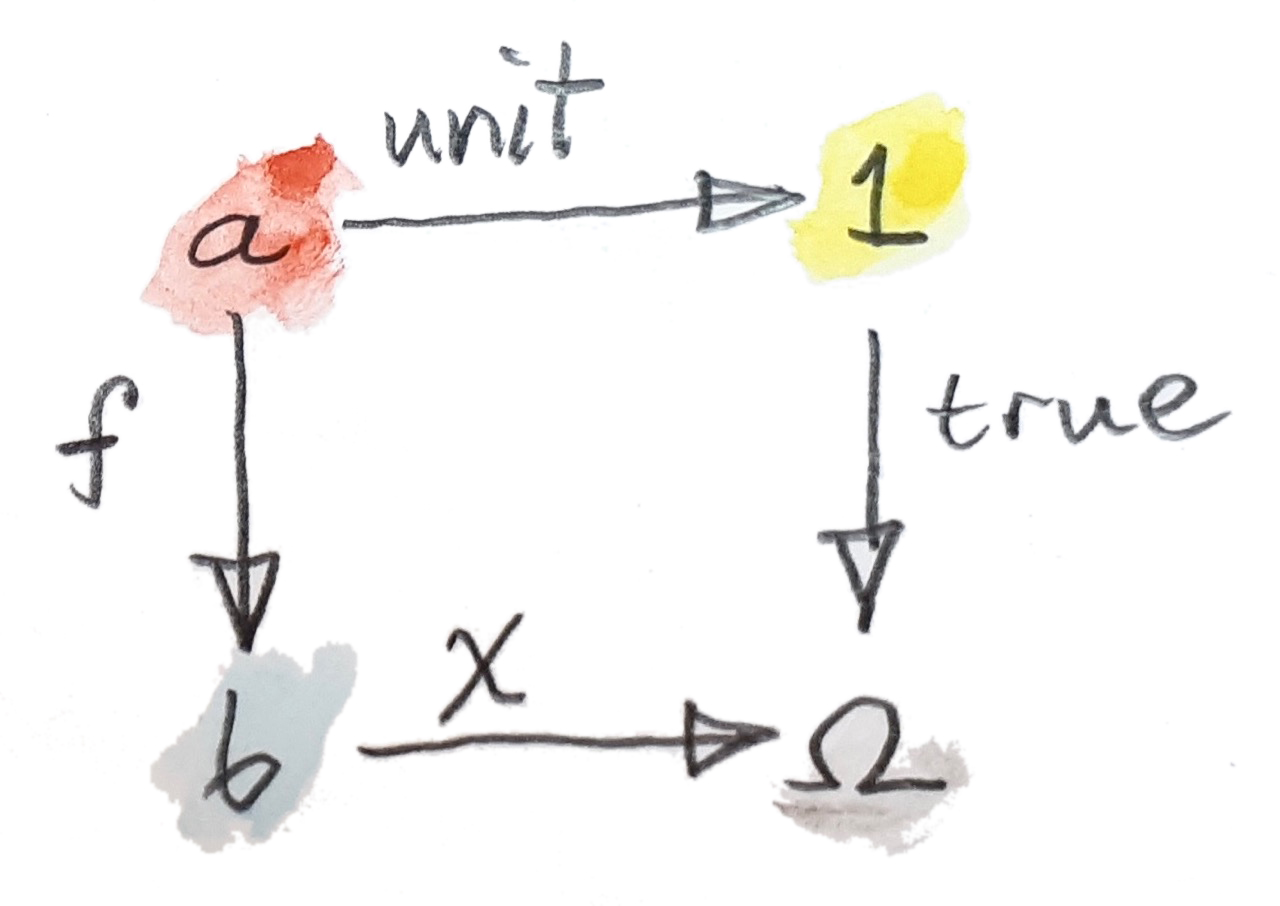
\includegraphics[width=2.41667in]{images/pullback.jpg}

Let's analyze this diagram. The pullback equation is:

\begin{verbatim}
true . unit = χ . f
\end{verbatim}

The function \texttt{true\ .\ unit} maps every element of \texttt{a} to
``true.'' Therefore \texttt{f} must map all elements of \texttt{a} to
those elements of \texttt{b} for which \texttt{χ} is ``true.'' These
are, by definition, the elements of the subset that is specified by the
characteristic function \texttt{χ}. So the image of \texttt{f} is indeed
the subset in question. The universality of the pullback guarantees that
\texttt{f} is injective.

This pullback diagram can be used to define the classifying object in
categories other than \textbf{Set}. Such a category must have a terminal
object, which will let us define the monomorphism \texttt{true}. It must
also have pullbacks --- the actual requirement is that it must have all
finite limits (a pullback is an example of a finite limit). Under those
assumptions, we define the classifying object \texttt{Ω} by the property
that, for every monomorphism \texttt{f} there is a unique morphism
\texttt{χ} that completes the pullback diagram.

Let's analyze the last statement. When we construct a pullback, we are
given three objects \texttt{Ω}, \texttt{b} and \texttt{1}; and two
morphisms, \texttt{true} and \texttt{χ}. The existence of a pullback
means that we can find the best such object \texttt{a}, equipped with
two morphisms \texttt{f} and \texttt{unit} (the latter is uniquely
determined by the definition of the terminal object), that make the
diagram commute.

Here we are solving a different system of equations. We are solving for
\texttt{Ω} and \texttt{true} while varying both \texttt{a} \emph{and}
\texttt{b}. For a given \texttt{a} and \texttt{b} there may or may not
be a monomorphism \texttt{f::a-\textgreater{}b}. But if there is one, we
want it to be a pullback of some \texttt{χ}. Moreover, we want this
\texttt{χ} to be uniquely determined by \texttt{f}.

We can't say that there is a one-to-one correspondence between
monomorphisms \texttt{f} and characteristic functions \texttt{χ},
because a pullback is only unique up to isomorphism. But remember our
earlier definition of a subset as a family of equivalent injections. We
can generalize it by defining a subobject of \texttt{b} as a family of
equivalent monomorphisms to \texttt{b}. This family of monomorphisms is
in one-to-one corrpespondence with the family of equivalent pullbacks of
our diagram.

We can thus define a set of subobjects of \texttt{b}, \texttt{Sub(b)},
as a family of monomorphisms, and see that it is isomorphic to the set
of morphisms from \texttt{b} to \texttt{Ω}:

\begin{verbatim}
Sub(b) ≅ C(b, Ω)
\end{verbatim}

This happens to be a natural isomorphism of two functors. In other
words, \texttt{Sub(-)} is a representable (contravariant) functor whose
representation is the object Ω.

\subsection{Topos}\label{topos}

A topos is a category that:

\begin{enumerate}
\tightlist
\item
  Is cartesian closed: It has all products, the terminal object, and
  exponentials (defined as right adjoints to products),
\item
  Has limits for all finite diagrams,
\item
  Has a subobject classifier \texttt{Ω}.
\end{enumerate}

This set of properties makes a topos a shoe-in for \textbf{Set} in most
applications. It also has additional properties that follow from its
definition. For instance, a topos has all finite colimits, including the
initial object.

It would be tempting to define the subobject classifier as a coproduct
(sum) of two copies of the terminal object --that's what it is in
\textbf{Set}--- but we want to be more general than that. Topoi in which
this is true are called Boolean.

\subsection{Topoi and Logic}\label{topoi-and-logic}

In set theory, a characteristic function may be interpreted as defining
a property of the elements of a set --- a \emph{predicate} that is true
for some elements and false for others. The predicate \texttt{isEven}
selects a subset of even numbers from the set of natural numbers. In a
topos, we can generalize the idea of a predicate to be a morphism from
object \texttt{a} to \texttt{Ω}. This is why \texttt{Ω} is sometimes
called the truth object.

Predicates are the building blocks of logic. A topos contains all the
necessary instrumentation to study logic. It has products that
correspond to logical conjunctions (logical \emph{and}), coproducts for
disjunctions (logical \emph{or}), and exponentials for implications. All
standard axioms of logic hold in a topos except for the law of excluded
middle (or, equivalently, double negation elimination). That's why the
logic of a topos corresponds to constructive or intuitionistic logic.

Intuitionistic logic has been steadily gaining ground, finding
unexpected support from computer science. The classical notion of
excluded middle is based on the belief that there is absolute truth: Any
statement is either true or false or, as Ancient Romans would say,
\emph{tertium non datur} (there is no third option). But the only way we
can know whether something is true or false is if we can prove or
disprove it. A proof is a process, a computation --- and we know that
computations take time and resources. In some cases, they may never
terminate. It doesn't make sense to claim that a statement is true if we
cannot prove it in finite amount of time. A topos with its more nuanced
truth object provides a more general framework for modeling interesting
logics.

Next:
\href{https://bartoszmilewski.com/2017/08/26/lawvere-theories/}{Lawvere
Theories}.

\subsection{Challenges}\label{challenges}

\begin{enumerate}
\tightlist
\item
  Show that the function \texttt{f} that is the pullback of
  \texttt{true} along the characteristic function must be injective.
\end{enumerate}
